\documentclass[letterpaper,10pt]{article}

\usepackage{titling}
\usepackage{listings}
\usepackage{url}
\usepackage{setspace}
\usepackage{subfig}
\usepackage{sectsty}
\usepackage{pdfpages}
\usepackage{colortbl}
\usepackage{multirow}
\usepackage{multicol}
\usepackage{relsize}
\usepackage{amsmath}
\usepackage{wasysym}
\usepackage{fancyvrb}
\usepackage{amssymb}
\usepackage{ifsym}
\usepackage{amsmath,amssymb,amsthm,graphicx,xspace}
\usepackage[titlenotnumbered,noend,noline]{algorithm2e}
\usepackage[compact]{titlesec}
\usepackage{XCharter}
\usepackage[T1]{fontenc}
\usepackage{tikz}
\usetikzlibrary{arrows,automata,shapes,trees,matrix,chains,scopes,positioning,calc}
\tikzstyle{block} = [rectangle, draw, fill=blue!20, 
    text width=2.5em, text centered, rounded corners, minimum height=2em]
\tikzstyle{bw} = [rectangle, draw, fill=blue!20, 
    text width=4em, text centered, rounded corners, minimum height=2em]

\definecolor{namerow}{cmyk}{.40,.40,.40,.40}
\definecolor{namecol}{cmyk}{.40,.40,.40,.40}

\let\LaTeXtitle\title
\renewcommand{\title}[1]{\LaTeXtitle{\textsf{#1}}}


\newcommand{\handout}[5]{
  \noindent
  \begin{center}
  \framebox{
    \vbox{
      \hbox to 5.78in { {\bf ECE356: Database Systems } \hfill #2 }
      \vspace{4mm}
      \hbox to 5.78in { {\Large \hfill #4  \hfill} }
      \vspace{2mm}
      \hbox to 5.78in { {\em #3 \hfill} }
    }
  }
  \end{center}
  \vspace*{4mm}
}

\newcommand{\lecture}[3]{\handout{#1}{#2}{#3}{Lecture #1}}
\newcommand{\tuple}[1]{\ensuremath{\left\langle #1 \right\rangle}\xspace}

\addtolength{\oddsidemargin}{-1.000in}
\addtolength{\evensidemargin}{-0.500in}
\addtolength{\textwidth}{2.0in}
\addtolength{\topmargin}{-1.000in}
\addtolength{\textheight}{1.75in}
\addtolength{\parskip}{\baselineskip}
\setlength{\parindent}{0in}
\renewcommand{\baselinestretch}{1.5}
\newcommand{\term}{Winter 2018}

\singlespace


\begin{document}

\lecture{ 9 --- Reduction to Relational Schema, Design Decisions }{\term}{Jeff Zarnett}

\section*{Modelling Diagrams into Tables}
If we have an entity-relation diagram, eventually we will want to turn that into a set of database tables. The conversion routine is not especially complicated and after a small amount of practice it is likely that you will be able to do it quickly and efficiently.

\paragraph{Strong Entity.} Strong entities are the easiest to turn into tables. The name of the table will be the name of the entity (surprise) and the attributes in the diagram become the attributes in the relation. The primary key in the table will be the same as the primary key in the diagram. If the diagram says an instructor has \textit{(id, name, salary)} and \textit{id} is the primary key, then the create table statement will assign types and lengths to these fields. 

\paragraph{Weak Entity.} Weak entities are more interesting. Suppose $A$ is a weak entity set and the strong attribute it depends on is $B$. The weak entity table is created using the attributes of $A$ as well as the primary key of $B$, the entity it depends upon. If the weak entity is the section of a course, as before, and course is the strong entity, then the section entity would be created with all attributes of the section (weak) entity and the primary key  of the course entity (course id).

It is also sensible to add constraints to this table that says the attribute(s) referencing the primary key of the strong entity  must exist in the strong entity table (not null and foreign key). In the weak entity table, the primary key is formed by the key referencing the strong entity plus the discriminator~\cite{dsc}.

Suppose that the weak entity is a list of something and the strong entity a container of some sort. Suppose you have a shipment: a single shipment is made up of items and those items are, let's say, weak entities in the example. Then the primary key would be the unique identifier of the shipment plus the discriminator, where the discriminator is an integer identifying the position in the list. So if the unique ID for a shipment is ABC12345, then the items for that shipment would have primary keys be \textit{(ABC12345, 0), (ABC12345, 1), (ABC12345, 2), (ABC12345, 3)...}. This also provides a nice way to sort them.

\paragraph{Relationships.} 
A relationship is possibly represented as a table in the database as well. As a first step, we will define the attributes for that table as if it will be a standalone table. Later, we might combine the table with another one to eliminate redundancy or simplify (see below) but for now the first step will be the naive table creation.

The table is created using (1) the primary key of each of the entities participating in the relationship, plus (2) any attributes that have been assigned to the relationship itself. That's pretty much it; the real question is what should form the primary key for this table? It depends on the nature of the relationship~\cite{dsc}:

\begin{itemize}
	\item For binary many-to-many relationships, the union of the primary keys of each entity participating in the set forms the primary key.
	\item For binary one-to-one relationships, the primary key of either set (but no need for both); either is fine.
	\item For binary many-to-one (or one-to-many) relationships, the primary key of the entity on the ``many'' side is the primary key for the relationship.
	\item For $n$-ary relationships where none of the relationships are ``to one'', the union of the primary key from participating entity sets makes up the primary key for the relationship.
	\item For $n$-ary relationships where there is a ``to one'' participant, the primary key is the union of primary keys of all the OTHER participating entities (but not the one that's ``to one''). 
\end{itemize}

The foreign key constraints should be added from the relationship table referencing the entities participating in the relationship. Now, some of the tables generated by this process are redundant and some can be combined to make things simpler and a little bit clearer...

\paragraph{Redundancy.}
Take a look at a relationship linking a weak entity to the corresponding strong entity. Weak entities are modelled as being many to one and the relationships have no descriptive attributes. Because the weak entity has the primary key of the related strong entity as one of its attributes (thanks the the relations being resolved into the entities it links). Thus, for this reason, a relation that specifically links the weak entity to the strong entity is fully redundant. 

Example: the weak entity of a section of a course linked to a strong entity of a course~\cite{dsc}. A section a section id, semester, and a year. It is related to a course that has a course ID. So when we have done the work of turning the relationship into some tables we'll find that the table for section we already have course ID as one of the attributes. So we would not need a table that actually links them anymore, as it would be totally redundant. 

\paragraph{Combination.}
Sometimes our diagram presents us a number of entities which we would like to combine when we are creating tables (and we'll see in an upcoming lecture whether this is a good idea or not). 

If a relationship exists between two tables $A$ and $B$ that is many-to-one (many $A$ correspond to one $B$), we might naively create tables for $A$, $B$, and one for the relation $AB$. If it is (almost) always the case that $A$ participates in the relation then we could actually combine $A$ and $AB$ to make a single relation that is the union of both attributes~\cite{dsc}. Or we might decide that means that $A$ simply gets an attribute that references $B$. If participation is not total, the use of null is appropriate.

The one-to-many relationship is just the reverse of the previous paragraph -- instead of adding the attribute(s) to $A$, add the attribute(s) to $B$ instead. In the case of a one-to-one relationship between $C$ and $D$, the attributes of the relation can be added to either one of the entities, $C$ or $D$, but not both. If we have a many-to-many relationship, then we cannot combine the tables (obviously). 

If we have combined two tables, then obviously, we don't need foreign keys to link them anymore (because, of course, it would make no sense). However, a foreign key that would have appeared on a relationship $AB$ that references some other entity needs to be created on the merged tables as well.

\paragraph{Generalization (Specialization).} To transform a generalization into an entity set, we have two choices. The most obvious approach is something along the lines of what Java will do in the background when you create a subclass of an object: the properties of the superclass appear on the subclass. Recall this diagram from earlier:

\begin{center}
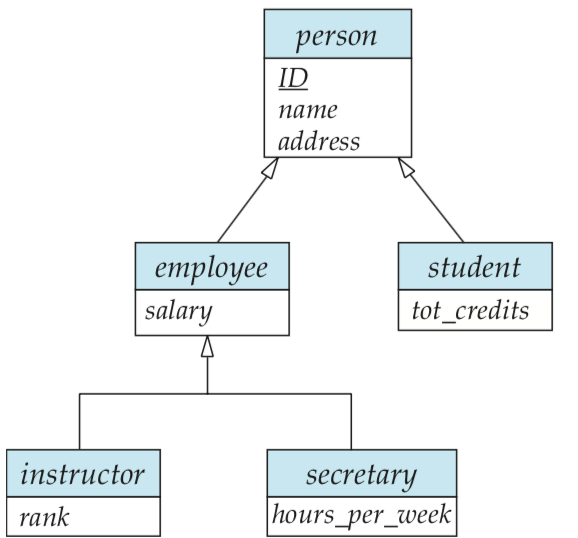
\includegraphics[width=0.35\textwidth]{images/specialization-generalization}\\
An E-R diagram showing specialization and generalization~\cite{dsc}.
\end{center}

In this case then we would define tables for instructor, secretary, and student. We might or might not have one for employee, depending on our rules. If, of course, we don't allow ``instantiation'' of a person, but instead a person must be either an employee or student, we would not create a table for the person relation. You may liken this decision to whether the class person is abstract or not.
So let's assume that instructor then created as \textit{(ID, name, address, salary, rank)} with \textit{ID} as the primary key. There will be some repetition here as the secretary relation will also have most of the attributes the same, except instead of rank it will have hours per week.

The alternative representation is to break it up so that we have instructor created as \textit{(ID, rank)}, which necessitates creating employee as \textit{(ID, salary)}, and person as \textit{(ID, name, address)}. This does require a fair amount of repetition in the primary key attribute since it will appear in all tables. The primary key is then the only one that is repeated. With some foreign keys set up to make the IDs match up, of course.

That's interesting, both of these things will have some redundancy. But how much will we have? Depends: if the generalization is both disjoint and complete, the first approach is better. Disjoint and complete means that no entity is a member of two lower-level entity sets directly below a higher-level set, and if every entity in the higher level set is in one of the lower-level sets~\cite{dsc}. If that's not the case, we might get some duplicate data, such as if a student can also be an employee: things like name and address appear twice for a person who is both. So perhaps the alternative approach is preferable if these two conditions do not hold.

\paragraph{Aggregation.} Aggregation is actually relatively easy to work out. The tables for the elements inside the aggregation are created as normal. Then the rules for creating the key constraints can just as easily be applied to any relationship that involves the aggregation. The primary key of the aggregation is the primary key of its defining set, so just use that (and no relation is created to specifically represent the aggregation)~\cite{dsc}.

\subsection*{Design Decisions}

In creating our E-R diagrams we have implicitly or explicitly made some key design decisions about how we would like to implement the design. In some cases there are better choices and worse choices, but in other cases there are alternatives that are equally valid that we could choose between.

\paragraph{Entity vs. Attribute.} A decision we need to make frequently is whether a new piece of data should be added as an attribute or as a new entity. Let's say we want to add an e-mail address to users.

If the relationship is anything other than 1:1 then it is very unlikely we will choose a new attribute. How many e-mail addresses are users allowed to have in the system? If it is just one, our decision is more interesting. If a user can have multiple e-mail addresses, we must choose a new entity to represent e-mails. What about letting multiple users share an e-mail address? We might not want to forbid that specifically (although we can), but it still takes us back to the decision of whether a user can have one e-mail address or many.

Let's assume that a user can have exactly one e-mail address. Then putting it in an attribute is a viable choice. What if we put it in another entity? That might not be the best choice here, because we would have an entity for e-mail address that contains nothing but the e-mail address and then the attribute to link it to the user. 

What if instead, we were thinking of adding multiple related fields instead of one field? Then it might make more sense to group those things separately in an entity of their own. An address, for example, is a number of related fields, street, city, postal code, et cetera. If a user has one address we could put all those fields on the user entity, but it might make more sense to move them to a different entity. Performance considerations may come into play (eventually) because large entities are unwieldy. 

But the real decision is more philosophical... What is an attribute and what is better as a set? There is not a bright line between the two and it may depend more on the real-life situation being modelled than any actual technical consideration.

There is a wrong choice, though, and that is using the primary key of an entity as an attribute of another, instead of a relationship~\cite{dsc}. Remember that in a relationship, in reality of course, the table will need to contain some reference to the other. But in the E-R diagram it should be represented as a relationship (especially because it allows the opportunity to assign more attributes to the relationship, that otherwise might not have been in the right place). Simply writing, for example, \textit{student\_id} as an attribute in a \textit{instructor} entity as an alternative way of showing that there is a relationship (advisor) is suboptimal.

It's also worth noting that a common mistake is to write redundant attributes on the relationship~\cite{dsc}. If a relationship is drawn between tables $r_{1}$ and $r_{2}$ in the diagram, there is no need to put the primary key of either $r_{1}$ or $r_{2}$ as attributes on that relation, because they are already implied by the fact that there exists a relationship between the two types. 

\paragraph{Entity vs. Relationship.} We are also sometimes faced with the decision about whether to make a particular object an entity or a relationship. There are things that are clearly an entity (e.g., a customer) and those that are clearly a relationship (e.g., a shopping cart) but there are other things that fall within a marginal category where it could go either way. In an online shopping scenario, though, what about order history? This is different from the idea of a shopping cart because if an item changes attributes before purchase, the data in the cart needs to be updated... if it changes after, for example, the price decreases, it does not change the already-purchased orders.

There are arguments for the relationship approach: it eliminates duplicate data and ensures that if a product is updated then the latest data is shown in the order. That might, actually, be an argument for the alternative. If a product is purchased then it might make sense to ``freeze'' in place some of its data at the time of purchase (e.g., price) so it is perhaps advisable to make an entity for a purchase order made. 

Another example in the university schema is what to do with registration: when a student takes a class should that be represented by a relation that says the student with the id $x$ registered in the section $y$? Consider the E-R diagram as below:

\begin{center}
	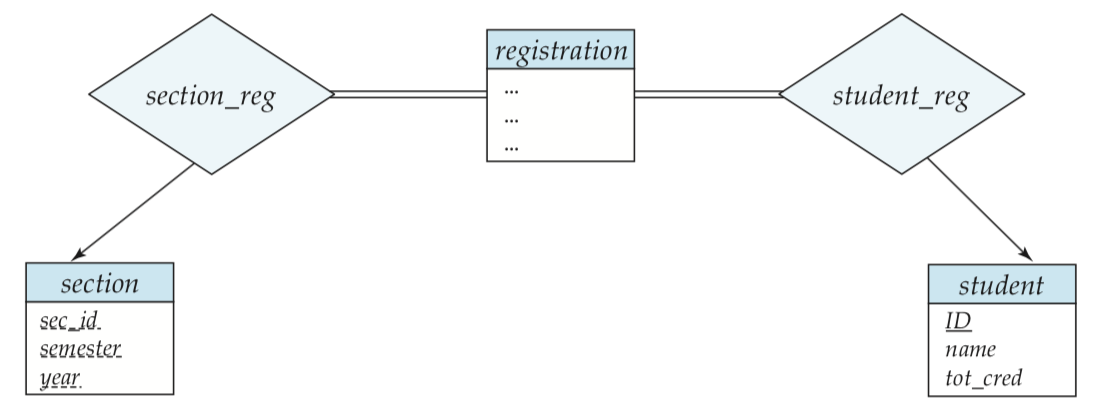
\includegraphics[width=0.7\textwidth]{images/reg-split}\\
	Registration entity created to replace a more complex relationship~\cite{dsc}.
\end{center}

My personal take on this is that this is worse than just representing student enrolment in a section as a simple relationship. This approach has more entities, more relationships, and is perhaps not as easily matched to a theoretical model of the university. That a student is registered in a course is less tangible than a shopping cart in the online shopping scenario, so it seems strange to make registration an entity. Then again, you could argue that registration corresponds to a card kept in a file somewhere but that is probably not how it really works (but the mysteries of the registrar's office are not for humans to know...).

\paragraph{Binary vs. Non-Binary Relationships.}
When we have a $n$-ary relationship, that is an $n$-way relationship such as we have seen before, we could choose instead to represent it as a number of binary relationships. Consider a work term report: it has an author (a student) and an evaluator (lab instructor). We could make it a three-way relationship or we could instead break it up into two relationships, one between work report and student, and one between work report and lab staff. If it was in one relationship, a work report that has no marker assigned yet would just have \texttt{null} as its assigned value until a marker is assigned.  

It is always possible to replace an $n$-ary relation with some number of binary relationships, although we may need to put an entity in the middle of it to make it all work out. Suppose we have a ternary (3 entity) relationship $R$ that connects entities $A$, $B$, and $C$. Any attributes of the ternary relationship become an entity $E$ and then three binary relations are created: $R_{A}$ relating $A$ and $E$, $R_{B}$ relating $B$ and $E$, and $R_{C}$ relating $C$ and $E$~\cite{dsc}.

\begin{center}
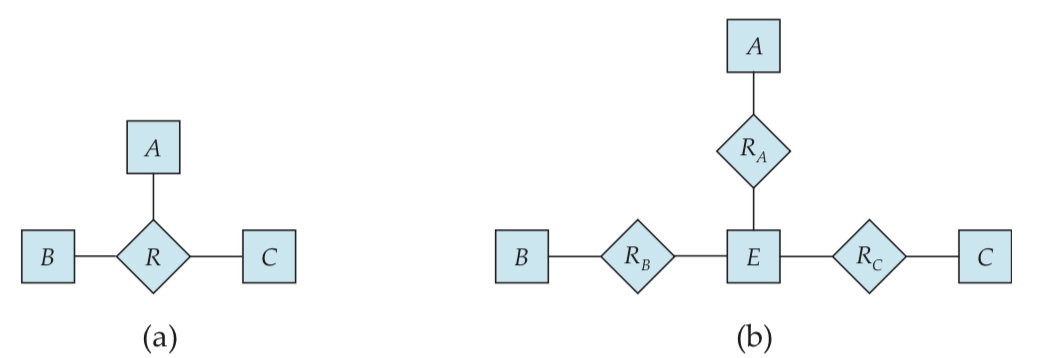
\includegraphics[width=0.7\textwidth]{images/ternary-to-binary}\\
Converting a ternary relationship (a) into three binary relationships (b)~\cite{dsc}.
\end{center}

Even though it is possible to turn a ternary relationship into binary relationships, there are reasons why this is undesirable. In fact, we can immediately consider three reasons why this is not always a great idea~\cite{dsc}:

\begin{itemize}
	\item When a single relationship is split into two or more, it may no longer be clear the split relationships have any connection. 
	\item An identifying attribute needs to be created for the new entity ($E$ in the above example) and this needs to be stored and maintained. Then there would be more relationships which would make the diagram more difficult to follow and ultimately also mean more tables that are created in the database.
	\item Constraints that exist in a ternary (or more) relationship may be difficult or impossible to express in binary relationships. If a constraint says the relationship is many-to-one from $(A, B)$ to $C$, i.e., each $AB$ pair is associated with at most one $C$ entity, this cannot be expressed with cardinality constraints on relations $R_{A}, R_{B}, R_{C}$.
\end{itemize}

\paragraph{Placement of Relationship Attributes.} 

In the case of one-to-one and one-to-many relationships we could choose to create a table for the relation, but we don't have to... We could instead associate the attributes of the relationship with one of the entities. If we have a work report entity and we want to relate it to its author, we could have a table that relates the two... or a work report entity might end up with an attribute for the student ID to connect the two. But this wouldn't work for a book and author relationship, because a book can have more than one author and an author can write more than one book.

This discussion takes us back full circle to the entity vs. relationship discussion from earlier. If the relationship to be modelled is a many-to-many relationship then there isn't really a lot of choice. If an attribute $A$ in the relationship is determined uniquely only by the combination of the entities' identifiers, then $A$ needs to be placed on that relationship and cannot be put on either side. If the relationship is a shopping cart in an online store, and a discount code has been applied, the discount code's application belongs neither to the customer nor any individual item in the cart.

\paragraph{Security.} Remember, permissions are handed out at the level of the table and that makes it sometimes necessary to divide some tables so that the appropriate security constraints can be applied. 

\paragraph{Conclusion.} There are, fortunately, some formal and precise ways for making a determination about whether our designs are appropriate. We would like our designs to be ``normal'' and there is a precise definition of what normal is. 

\bibliographystyle{alphaurl}
\bibliography{356}


\end{document}
